%# -*- coding: utf-8-unix -*-
\chapter{船舶兴波流动势的计算方法}
\label{chap:fsG}

\section{基本边界积分表达式}
\label{sec:bdryint}
考虑被封闭表面$\Sigma$包围的有限三维区域$\mathcal{D}$。域内或边界面上的点
为$\bm{\xi}\equiv(\xi,\eta,\zeta)$,点$\bm{\xi}\in\Sigma$处
垂直于表面$\Sigma$并指向域内的单位法向量为
$\mathbf{n}\equiv\mathbf{n}(\bm{\xi})$。

考虑定义在$\bm{\xi}\in\mathcal{D}\bigcup\Sigma$上的可微标量场
$\phi(\bm{\xi})$和$\psi(\bm{\xi})$。由Green第二公式得
\begin{equation}
  \int_\mathcal{D}\mathrm{d}v\,(\phi\nabla^2_\mathbf{\xi}\psi
  -\psi\nabla^2_{\mathbf{\xi}}\phi)
  =\int_\Sigma\mathrm{d}a\,\mathbf{n}\cdot(
  \psi\nabla_\mathbf{\xi}\phi
  -\phi\nabla_\mathbf{\xi}\psi
  )
  \label{eq:greentheorem}
\end{equation}
此处,$\nabla_\bm{\xi}$和$\nabla^2_\bm{\xi}$为
\begin{eqnarray}
  &\nabla_\mathbf{\xi}\equiv(\frac{\partial}{\partial\xi},
  \frac{\partial}{\partial\eta},\frac{\partial}{\partial\zeta})
  \label{eq:diff}\\
  &\nabla^2_\mathbf{\xi}\equiv\nabla_\mathbf{\xi}\cdot\mathbf{\xi}
  \equiv\frac{\partial^2}{\partial\xi^2}+\frac{\partial^2}{\partial\eta^2}
  +\frac{\partial^2}{\partial\zeta^2}\label{eq:laplace}
\end{eqnarray}
$\mathrm{d}v\equiv \mathrm{d}(\xi)$和$\mathrm{d}a=\mathrm{d}a(\xi)$是点
$\bm{\xi}\in\mathcal{D}$或$\bm{\xi}\in\Sigma$处的体积微元和面积微元。

取$\phi$为速度势,$\psi=G(\mathbf{x},\bm{\xi})$,这里
$G(\mathbf{x},\bm{\xi})$称作Green函数,满足Poisson方程
\begin{equation}
  \nabla^2_\mathbf{\xi}G=\delta(\xi-x)\delta(\eta-y)\delta(\zeta-z)
  \label{eq:Gdef}
\end{equation}
这里$\delta(\xi-x)$、$\delta(\eta-y)$、$\delta(\zeta-z)$是Dirac函数。
由$\nabla^2_{\bm{\xi}}\phi=0$、\eqref{eq:greentheorem}、\eqref{eq:Gdef}和
Dirac函数的性质得
\begin{eqnarray}
  \widetilde{C}\widetilde{\phi}=
  \int_\Sigma\mathrm{d}a\,(
  G\mathbf{n}\cdot\nabla_\mathbf{\xi}\phi
  -\phi\mathbf{n}\cdot\nabla_\mathbf{\xi}G
  )
  \label{eq:bdryint}
\end{eqnarray}
这里$\widetilde{\phi}\equiv\phi(\mahbf{x})$,当$\mathbf{x}\in\mathcal{D}$时取
$\widetilde{C}=1$,
当$\mathbf{x}\in\Sigma$时取$\widetilde{C}=1/2$,当$\mathbf{x}\notin\mathcal{D}$时取$\widetilde{C}=0$。当$\mathbf{x}\in\Sigma$时,表达式\eqref{eq:bdryint}只包含
$\phi$和它的法向导数$\mathbf{n}\cdot\nabla_{\bm{\xi}}\phi$在边界$\Sigma$上的值,
因此提供了确定$\phi$在边界$\Sigma$上值的(积分)方程。

式\eqref{eq:bdryint}将三维区域内点$\mathbf{x}$处的速度势$\phi(\mathbf{x})$
用$\phi(\mathbf{x})$和它的法向导数$\mathbf{n}\cdot\nabla_{\bm{\xi}}\phi=
\partial\phi/\partial n$在表面$\Sigma$上的值表示。因此,边界积分表达式
\eqref{eq:bdryint}将问题从三维降为二维。

\section{基本Green函数}
\label{sec:rankinesource}

满足Poisson方程\eqref{eq:Gdef}的一个Green函数是
\begin{equation}
  4\pi G=-1/r
  \label{eq:rankinesource}
\end{equation}
这里
\begin{equation}
  r\equiv\sqrt{(x-\xi)^2+(y-\eta)^2+(z-\zeta)^2}
  \label{eq:r}
\end{equation}
是点$\mathbf{x}=(x,y,z)$到点$\bm{\xi}=(\xi,\eta,\zeta)$之间的距离。
可以验证,$G$满足
\begin{equation}
  \nabla^2_{\bm{\xi}}G=0\quad\text{如果}\quad r>0
  \label{eq:laplaceG}
\end{equation}
与\eqref{eq:Gdef}一致。

注意到Green函数\eqref{eq:rankinesource}即满足Poisson方程\eqref{eq:Gdef}也满足如下
的Poisson方程
\begin{equation}
  \nabla^2_{\mathbf{x}}G\equiv(\partial^2/\partial x^2+\partial^2/\partial y^2
  +\partial^2/\partial z^2)G=\delta(x-\xi)\delta(y-\eta)\delta(z-\zeta)
  \label{eq:Gphyintrp}
\end{equation}
这表明Green函数\eqref{eq:rankinesource}可以看作位于点$\bm{\xi}$的单位点源在
场点$\mathbf{x}$处产生的速度势。
这种将$\mathbf{x}$看作场点和将$\bm{\xi}$看作源点的理解通常被采用。这表明
由边界积分表达式\eqref{eq:bdryint}定义的域$\mathcal{D}$内或边界面$\Sigma$上的
调和函数$\phi(\mathbf{x})$可以用分布在边界面$\Sigma$上的点源$G$和偶极子$\mathbf{n}\cdot\nabla_{\bm{\xi}}G$表示,并且点源和偶极子的强度分别等于$\mathbf{n}\cdot\nabla_{\bf{\xi}}\phi$和$\phi$。



\section{自由面Green函数}
\label{sec:fsG}

满足Poisson方程\eqref{eq:Gdef}的Green函数不是唯一的。事实上,任何形如
\begin{equation}
  4\pi G=-1/r+H,\quad\text{其中}\quad \nabla^2_{\bm{\xi}}H=0,\quad\text{对于}
  \quad\bm{\xi}\in\mathcal{D}
  \label{eq:generalG}
\end{equation}
的Green函数都满足Poisson方程\eqref{eq:Gdef}。

对于船在无限深广的静水中匀速前进的问题,边界积分表达式中的积分边界$\Sigma$
可取为
\begin{equation}
  \Sigma=\Sigma^H+\Sigma^F+\Sigma^\infty
  \label{eq:bdry}
\end{equation}
其中$\Sigma_a^H$代表平均船体湿表面,$\Sigma^F$代表位于船体表面外的平均自由面,
$\Sigma^\infty$代表包含流场$\mathcal{D}$的半径趋于无穷大的下半球面。

我们在第?章推导了船在无限深广的静水中匀速前进的速度势$\phi$满足的定解条件。
为了方便本章应用,现重新列出如下
\begin{subequations}\label{eq:govreiter}
  \begin{eqnarray}
  &&\nabla^2_{\bm{\xi}}\phi\equiv
  (\partial^2/\partial\xi^2+\partial^2/\partial\eta^2+\partial^2/\partial\zeta^2)\phi=0,\quad \bm{\xi}\in\mathcal{D}\label{eq:govreiter-a}\\
  &&[\partial/\partial\zeta+(F\partial/\partial\xi-\epsilon)^2]\phi=0,\quad\bm{\xi}
  \in\Sigma^{F}\label{eq:govreiter-fs}\\
  &&\mathbf{n}\cdot\nabla_{\bf{\xi}}\phi=n_x, \quad \bm{\xi}\in\Sigma^H
  \label{eq:govreiter-hull}\\
  &&\phi\rightarrow0, \quad \bm{\xi}\in\Sigma^\infty
  \label{eq:govreiter-far}
\end{eqnarray}
\end{subequations}

当$r\to\infty$时,基本Green函数\eqref{eq:rankinesource}的量阶是$\mathcal{O}(1/r)$.
而$\mathbf{n}\cdot\nabla_{\bm{\xi}}\phi$的量阶是$\mathcal{O}(\phi/r)$,因此
$G\mathbf{n}\cdot\nabla_{\bm{\xi}}\phi$的量阶是$\mathcal{O}(\phi/r^2)$。
同理可知,基本边界积分表达式\eqref{eq:bdryint}中整个被积函数的量阶为
$\mathcal{O}(\phi/r^2)$。无穷远表面积的量纲是$\mathcal{O}(r^2)$。
由此可知当$r\to\infty$时,边界积分表达式\eqref{eq:bdryint}在$\Sigma^\infty$的
积分值为零。

由边界积分表达式\eqref{eq:bdryint}、积分边界\eqref{eq:bdry}、
速度势船体表面边界条件\eqref{eq:govreiter-hull},考虑远场$\Sigma^{\infty}$对
边界积分表达式\eqref{eq:bdryint}的影响得
\begin{equation}
  \tilde\phi=\int_{\Sigma^H}(Gn^x-\phi\mathbf{n}\cdot\nabla G)\,\mathrm{d}a
  +\int_{\Sigma^F}(\phi G_{\zeta}-G\phi_{\zeta})\,\mathrm{d}\xi\mathrm{d}\eta
  \label{eq:bdryintmean}
\end{equation}

如果我们选择的Green函数满足如下齐次自由面边界条件
\begin{equation}
  [\partial/\partial\zeta+(\epsilon+F\partial/\partial\xi)^2]G=0, \quad \zeta=0
  \label{eq:Gbdry-fs}
\end{equation}
则由式\eqref{eq:govreiter-fs}、\eqref{eq:Gbdry-fs}可知
\begin{equation}
  \phi G_{\zeta}-\G\phi_{\zeta}=F^2(G\phi_{\xi}-\phi G_{\xi})_{\xi}
  \label{eq:fsintegrand}
\end{equation}
由此可知
\begin{eqnarray}
  \int_{\Sigma^F}\mathrm{d}\xi\mathrm{d}\eta\,
  (\phi G_{\zeta}-G\phi_{\zeta})
  &=&F^2\int_{\Gamma}(G\phi_\xi-\phi G_\xi)\,\mathrm{d}\eta \nonumber\\
  &=&F^2\int_{\Gamma}(G\phi_{\xi}-\phi G_{\xi})t^y\mathrm{d}\ell
  \label{eq:watr}
\end{eqnarray}
这里使用了Stokes定理将在自由面$\Sigma^F$上的积分转化为在平均水线$\Gamma$上的线积分。
这里水线$\Gamma$的方向(从上往下看)为顺时针方向,$\mathrm{d}\ell$是水线$\Gamma$的
弧长微元,$\mathbf{t}\equiv (t^x,t^y,0)$是水线$\Gamma$的单位切向量。
因此在左舷$y\ge0$,$\mathbf{t}$指向船首,我们有$\mathbf{t}=(n^y,-n^x,0)/\sqrt{(n^x)^2+(n^y)^2}$,其中$\mathbf{n}=(n^x,n^y,n^z)$是船体曲面的外法向量(指向水中)。


通过选择\eqref{eq:generalG}中调和函数$H$,可使Green函数$G$满足自由面边界条件
\eqref{eq:Gbdry-fs}。此Green函数还满足下半平面$\zeta<0$内的Poisson方程
\eqref{eq:Gdef}和无穷远条件:当$r\to\infty$时,$G\to0$。
因此Green函数$G(\mathbf{x},\bm{\xi})$是下述问题的解
\begin{subequations}\label{eq:Gbdry}
  \begin{eqnarray}
    &&\Delta^2_{\bm{\xi}}G=\delta(\xi-x)\delta(\eta-y)\delta(\zeta-z),\quad \zeta<0
    \label{eq:Gbdrygov}\\
    &&G\to0,\quad r\to\infty\label{eq:Gbdryfar}\\
    &&[\partial/\partial\zeta+(\epsilon+F\partial/\partial\xi)^2]G=0,\quad \zeta=0
    \label{eq:Gbdryfs}
  \end{eqnarray}
\end{subequations}

满足问题\eqref{eq:Gbdry}的一般解为
\begin{equation}
  4\pi G=-1/r+1/r'+P/\pi
  \label{eq:fsGgeneral}
\end{equation}
这里
\begin{equation}
  r'=\sqrt{(x-\xi)^2+(y-\eta)^2+(z-\zeta)^2}
  \label{eq:r'}
\end{equation}
是点$\bm{\xi}=(\xi,\eta,\zeta)$到点$\mathbf{x}=(x,y,z)$关于自由面$\zeta=0$的镜像
$\mathbf{x'}=(x,y,-z)$的距离。函数$1/r'$满足下半平面$\zeta<0$内的Laplace方程。

函数$P$是下述问题的解
\begin{subequations}\label{eq:Pbdry}
  \begin{eqnarray}
    &&\nabla^2_{\bm{\xi}}P=0,\quad \zeta<0\label{eq:Pbdrygov}\\
    &&P\to 0,\quad r\to\infty\label{eq:Pbdryfar}\\
    &&[\partial/\partial\zeta+(\epsilon+F\partial/\partial\xi)^2]P
    =-2\pi\partial(1/r')/\partial\zeta,\quad \zeta=0
    \label{eq:Pbdryfs}
  \end{eqnarray}
\end{subequations}
式\eqref{eq:fsGgeneral}将Green函数分为基本Green函数$-1/r$和另外两部分的和。
$1/r'$对应于将自由面边界条件取为$G=0$,这相当于在\eqref{eq:Gbdryfs}中$F\to\infty$。
$P$考虑了自由面边界的效应。

由边界条件\eqref{eq:Pbdryfs}和式\eqref{eq:r'}可得,调和函数$P$只依赖于
\begin{equation}
  x-\xi,\quad y-\eta,\quad z+\zeta
  \label{eq:3var}
\end{equation}
三个变量。
另外,由式\eqref{eq:fsGgeneral}可知在自由面$\zeta=0$上$r=r'$,因此Green函数只依赖于
变量$x-\xi$,$y-\eta$,$z+\zeta$。因此,自由面条件\eqref{eq:Gbdryfs}也可以写作
如下等价形式
\begin{equation}
  [\partial/\partial z+(F\partial/\partial x-\epsilon)^2]G=0
  \label{eq:Gbdryfs-b}
\end{equation}
而Poisson方程\eqref{eq:Gbdrygov}也可表示成等价形式\eqref{eq:Gphyintrp}。
因此Green函数也是下述问题的解
\begin{subequations}\label{eq:fsG}
  \begin{eqnarray}
    && (\partial^2/\partial x^2+\partial^2/\partial y^2+\partial^2/\partial z^2)G=\delta(x-\xi)\delta(y-\eta)\delta(z-\zeta),\quad z<0
    \label{eq:fsGgov}\\
  &&[\partial/\partial z+(F\partial/\partial x-\epsilon)^2]G=0,\quad z=0
  \label{eq:fsGfs}\\
  && G\to\infty,\quad r\to\infty \label{eq:fsGfar}
  \end{eqnarray}
\end{subequations}

式\eqref{eq:fsG}表明,Green函数$G(\mathbf{x},\bm{\xi})$可看作存在自由面时,
位于$\bf{\xi}$的点源在场点$\mathbf{x}$处产生的速度势。

\section{双重积分形式Green函数}
\label{sec:fsGiint}

下面求解满足\eqref{eq:Gbdry}的Green函数。此Green函数的形式为\eqref{eq:fsGgeneral},
其中函数$P$是满足\eqref{eq:Pbdry}的解。通过对坐标$\xi$和$\eta$进行双Fourier变换
可求得函数$P$。

记$1/r$的Fourier变换为$(1/r)^*$。
考虑到$1/r$满足Poisson方程,即
\begin{equation}
  (\partial^2/\partial\xi^2+\partial^2/\partial\eta^2+\partial^2/\partial\zeta^2)
  (1/r)=-4\pi\delta(\xi-x)\delta(\eta-y)\delta(\zeta-z)
  \label{eq:req}
\end{equation}
对\eqref{eq:req}进行Fourier变换得
\begin{equation}
  \mathrm{d}^2(1/r)^*/\mathrm{d}\zeta^2-k^2(1/r)^*=-2\mathrm{e}^{-\mathrm{i}(\alpha x+\beta y)}\delta(\zeta-z)
  \label{eq:reqft}
\end{equation}
其中$k^2=\alpha^2+\beta^2$。微分方程\eqref{eq:reqft}的通解为
\begin{equation*}
  (1/r)^*=A^{+}\mathrm{e}^k\zeta+A^{-}\mathrm{e}^{-k\zeta}
\end{equation*}
其中$A^+$与$A^-$为常数。由于$1/r$是$\zeta-z$的偶函数,且当$\zeta-z\to\pm\infty$时
趋于零,所以$(1/r)^*$可表示为
\begin{equation}
  (1/r)^*=A\mathrm{e}^{-k|\zeta-z|}
  \label{eq:rftgen-b}
\end{equation}
其中$A$为未知常数。

由式\eqref{eq:rftgen-b}定义的函数$(1/r)^*$在$\zeta=z$处连续且等于$A$。
而它的导数在$\zeta=z$不连续。特别地,导数$\mathrm{d}(1/r)^*/\mathrm{d}\zeta)$为
\begin{equation*}
  \frac{\mathrm{d}(1/r)^*}{\mathrm{d}\zeta}=
  \left\{
    \begin{array}{ll}
      kA\mathrm{e}^{k(\zeta-z)}, & \zeta<z \\
      -kA\mathrm{e}^{-k(\zeta-z)}, & z<\zeta
    \end{array}
    \right.
\end{equation*}
由此可知
\begin{equation}
  \frac{\mathrm{d}(1/r)^*}{\mathrm{d}\zeta}=
  \left\{
    \begin{array}{ll}
      kA, & \zeta=z-0 \\
      -kA, & \zeta=z+0
    \end{array}
    \right.
  \label{eq:drdzcoin}
\end{equation}
将式\eqref{eq:reqft}对$\zeta$在区间$[z-0,z+0]$进行积分得
\begin{equation*}
  [\mathrm{d}(1/r)^*/\mathrm{d}\zeta]|^{z+0}_{z-0}-k^2\int_{z-0}^{z+0}
  \mathrm{d}\zeta\,(1/r)^*=-2\mathrm{e}^{-\mathrm{i}(\alpha x+\beta y)}
\end{equation*}
由此式和式\eqref{eq:drdzcoin}可得
$-2kA=-2\mathrm{e}^{-\mathrm{i}(\alpha x+\beta y)}$。因此
\begin{equation*}
  A=\mathrm{e}^{-\mathrm{i}(\alpha x+\beta y)}/k
\end{equation*}
由此式和式\eqref{eq:rftgen-b}得
\begin{equation}
(1/r)^*=\mathrm{e}^{-k|z-\zeta|-\mathrm{i}(\alpha x+\beta y)}/k
  \label{eq:rft}
\end{equation}

考虑到$1/r'$是点$\bm{\xi}\equiv(\xi,\eta,\zeta)$到点$\mathbf{x}\equiv(x,y,z)$关于
$\zeta=0$的镜像点$\mathbf{x'}\equiv(x,y,-z)$的距离。在式\eqref{eq:rft}中将$z$
替换为$-z$并注意到$(z+\zeta)< 0$可得
\begin{equation}
  (1/r')^*=\mathrm{e}^{k(z+\zeta)-\mathrm{i}(\alpha x+\beta y)}/k,\quad z<0\quad\text{且}\quad\zeta<0
  \label{eq:r'ft}
\end{equation}

函数$P$的Fourier变换为
\begin{equation}
  P^*(\alpha,\beta,\zeta;\mathbf{x})=\frac{1}{2\pi}\int_{-\infty}^{\infty}
  \mathrm{d}\eta\int_{-\infty}^{\infty}\mathrm{d}\xi\,\mathrm{e}^{-\mathrm{i}(\alpha\xi+\beta\eta)}P(\xi,\eta,\zeta;\mathbf{x})
  \label{eq:Pfourier}
\end{equation}
其逆变换为
\begin{equation}
  P(\xi,\eta,\zeta;\mathbf{x}})=\frac{1}{2\pi}\int_{-\infty}^{\infty}
  \mathrm{d}\beta\int_{-\infty}^{\infty}\mathrm{d}\alpha\,\mathrm{e}^{\mathrm{i}(\alpha\xi+\beta\eta)}P^*(\alpha,\beta,\zeta;\mathbf{x})
  \label{eq:Pfourierinv}
\end{equation}

对\eqref{eq:Pbdry}进行Fourier变换可得
\begin{subequations}\label{eq:Peqft}
  \begin{eqnarray}
    && \mathrm{d}^2P^*/\mathrm{d}\zeta^2-k^2P^*=0,\quad -\infty<\zeta<0
    \label{eq:Peqftgov}\\
    && P^*\to 0,\quad \zeta\to -\infty\label{eq:Peqftfar}\\
    && \mathrm{d}P^*/\mathrm{d}\zeta-[F^2\alpha^2-2\mathrm{i}\epsilon F\alpha-\epsilon^2]P^*=-2\pi\mathrm{e}^{kz-\mathrm{i}(\alpha x+\beta y)},\quad \zeta=0
    \label{eq:Peqftfs}
  \end{eqnarray}
\end{subequations}
微分方程\eqref{eq:Peqft}的通解为
\begin{equation}
  P^*=A^{+}\mathrm{e}^{k\zeta}+A^{-}\mathrm{e}^{-k\zeta}
  \label{eq:Pftgen}
\end{equation}
其中$A^{+}$与$A^{-}$为常数。由边界条件\eqref{eq:Peqftfar}可知$A^{-}=0$。
由边界条件\eqref{eq:Peqftfs}可得解为
\begin{equation}
  P^*=2\pi\mathrm{e}^{k(z+\zeta)-\mathrm{i}(\alpha x+\beta y)}/[k-(F\alpha-\mathrm{i}\epsilon)^2]
  \label{eq:Pft}
\end{equation}
由\eqref{eq:Pfourierinv}得
\begin{equation}
  P=-\int_{-\infty}^{\infty}\mathrm{d}\beta\int_{-\infty}^{\infty}\mathrm{d}\alpha\,
  \frac{\mathrm{e}^{k(z+\zeta)-\mathrm{i}[\alpha(x-\xi)+\beta(y-\eta)]}}{k-(F\alpha-\mathrm{i}\epsilon)^2}
  \label{eq:Piint}
\end{equation}

由\eqref{eq:generalG}和式\eqref{eq:Piint}得
\begin{equation}
  4\pi G=\frac{-1}{r}+\frac{1}{r'}-\frac{1}{\pi}
  \int_{-\infty}^{\infty}\mathrm{d}\beta\int_{-\infty}^{\infty}\mathrm{d}\alpha\,
  \frac{\mathrm{e}^{k(z+\zeta)-\mathrm{i}[\alpha(x-\xi)+\beta(y-\eta)]}}{k-(F\alpha-\mathrm{i}\epsilon)^2}
  \label{eq:Giint}
\end{equation}
这是双重积分形式的线性自由表面兴波Green函数。但由于累次积分形式Green函数难于处理,
下面将给出单重积分形式的Green函数,以便于分析和数值计算。

\section{单重积分形式Green函数}
\label{sec:Gint}

记$x'=x-\xi$,$y'=y-\eta$,$z'=z+\zeta$,双重积分形式Green函数\eqref{eq:Giint}
可改写为
\begin{equation}
  4\pi G=\frac{-1}{r}+\frac{1}{r'}-\frac{1}{\pi}\int_{-\infty}^{\infty}
  \mathrm{e}^{-\mathrm{i}y'\beta}I_1(\beta,x',z',\epsilon)\,\mathrm{d}\beta
  \label{eq:inti1}
\end{equation}
其中,$I_1$为
\begin{equation}
  I_1(\beta;x',z',\epsilon)=\int_{-\infty}^{\infty}
  \frac{\mathrm{e}^{\sqrt{\alpha^2+\beta^2}z'-\mathrm{i}\alpha x'}}{\sqrt{\alpha^2+\beta^2}-(\alpha-\mathrm{i}\epsilon)^2}\,
  \mathrm{d}\alpha
  \label{eq:I1}
\end{equation}

$I_1$的被积函数有两个一阶极点,它们是方程
$\sqrt{\alpha^2+\beta^2}=(\alpha-\mathrm{i}\epsilon)^2$的根。
求解该方程可知当$\epsilon\to 0$时,两根为$\pm s+\mathrm{i}0$,即方程的根
从上半平面趋于$\pm s$。这里
\begin{equation}
  s=\sqrt{\frac{1+\sqrt{1+4\beta^2}}{2}}
  \label{eq:2poles}
\end{equation}
极点的位置在图\ref{fig:cntrint}中表出。可把积分$I_1$看作包含实轴的围道积分在实轴上的积分。
由于$\sqrt{\alpha^2+\beta^2}$是$\alpha$平面上的多值函数,其支点为
$\alpha=\pm\mathrm{i}|\beta|$,为了得到单值分支,需要将$\alpha$平面沿支割线
割破。这里支割线选为$\alpha=\mathrm{i}\alpha_i$,其中$-\infty<\alpha_i<-|\beta|$
或$|\beta|<\alpha_i<\infty$,对应于将复变函数$\sqrt{z}$的支割线选为$z<0$。
支割线的位置在图\ref{fig:cntrint}中表出。
要使用围道积分,需满足条件
\begin{equation*}
  \mathrm{Re}[z'\sqrt{\alpha^2+\beta^2}-\mathrm{i}x'\alpha]\le 0,
  \quad |\alpha|\to\infty
\end{equation*}
此时显然有
\begin{equation}
  \lim_{|\alpha|\to\infty}\frac{\alpha\mathrm{e}^{\sqrt{\alpha^2+\beta^2}z'-\mathrm{i}\alpha x'}}{\sqrt{\alpha^2+\beta^2}-(\alpha-\mathrm{i}\epsilon)^2}=0
  \label{eq:intcntr}
\end{equation}
可以验证,图\ref{fig:cntrint}所示的围道积分满足该条件。
\begin{figure}[htp]
  \centering
  \captionstyle{\centering}
  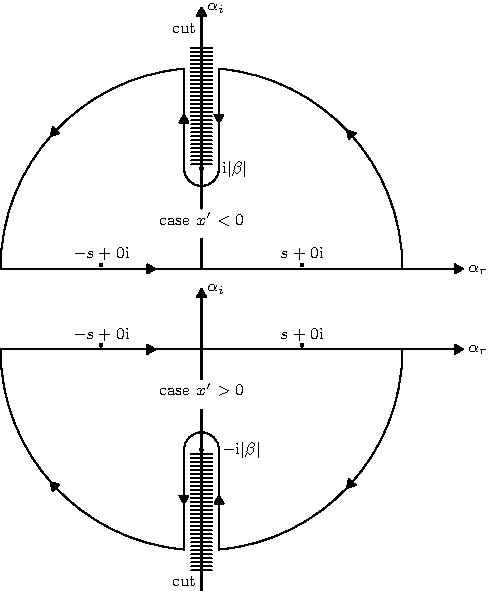
\includegraphics[width=0.5\textwidth]{chap4/contour_int.pdf}
  \bicaption[fig:cntrint]{复平面$\alpha=\alpha_r+\mathrm{i}\alpha_i$上的积分围道}
  {复平面$\alpha=\alpha_r+\mathrm{i}\alpha_i$上当$x'<0$和$x'>0$时的积分围道}{Fig}
  {Integration contours in the complex $\alpha=\alpha_r+\mathrm{i}\alpha_i$
plane for $x'<0$ and $x'>0$}
\end{figure}

首先考虑$x'>0$的情形。在支割线$\alpha_r=0,-\infty<\alpha_i<-|\beta|$的两边
$\alpha=\pm 0+\mathrm{i}\alpha_i$,我们有$\sqrt{\alpha^2+\beta^2}=\mp\mathrm{i}\sqrt{\alpha_i^2-\beta^2}$。在对应$x'>0$的围道内被积函数解析,考虑到式\eqref{eq:intcntr}
,由Cauchy积分定理得
\begin{equation*}
  I_1+\int_{-\infty}^{-|\beta|}
  \frac{\mathrm{e}^{\alpha_i x'-\mathrm{i}\sqrt{\alpha_i^2-\beta^2}z'}}{\alpha_i^2-
    \mathrm{i}\sqrt{\alpha_i^2-\beta^2}}\mathrm{i}\,\mathrm{d}\alpha_i
  +\int_{-|\beta|}^{-\infty}
  \frac{\mathrm{e}^{\alpha_i x'+\mathrm{i}\sqrt{\alpha_i^2-\beta^2}z'}}{\alpha_i^2+
    \mathrm{i}\sqrt{\alpha_i^2-\beta^2}}\mathrm{i}\,\mathrm{d}\alpha_i=0
\end{equation*}
将上式两个积分项移到等式右边,整理得
\begin{equation*}
  I_1=\int_{-\infty}^{-|\beta|}
  \frac{\mathrm{e}^{\alpha_i x'+\mathrm{i}\sqrt{\alpha_i^2-\beta^2}z'}}{\alpha_i^2+
    \mathrm{i}\sqrt{\alpha_i^2-\beta^2}}\mathrm{i}\,\mathrm{d}\alpha_i
  +\int_{-|\beta|}^{-\infty}
  \frac{\mathrm{e}^{\alpha_i x'-\mathrm{i}\sqrt{\alpha_i^2-\beta^2}z'}}{\alpha_i^2-
    \mathrm{i}\sqrt{\alpha_i^2-\beta^2}}\mathrm{i}\,\mathrm{d}\alpha_i
\end{equation*}
对上式第一个积分项和第二个积分项分别作变量代换$\mu=\sqrt{\alpha_i^2-\beta^2}$和
$\mu=-\sqrt{\alpha_i^2-\beta^2}$得
\begin{equation}
  I_1=\mathrm{i}\int_{-\infty}^{\infty}
  \frac{\mathrm{e}^{-x'\sqrt{\mu^2+\beta^2}+\mathrm{i}\mu z'}}{(\mu^2+\beta^2+\mathrm{i}\mu)\sqrt{\mu^2+\beta^2}}\mu\,\mathrm{d}\mu
  \label{eq:I1mu-a}
\end{equation}

下面考虑$x'<0$的情形。在支割线$\alpha_r=0,|\beta|<\alpha_i<\infty$的两边
$\alpha=\pm 0+\mathrm{i}\alpha_i$,
我们有$\sqrt{\alpha^2+\beta^2}=\pm\mathrm{i}\sqrt{\alpha_i^2-\beta^2}$。
在对应$x'<0$的围道内被积函数有两个一阶极点$\alpha=\pm s$,考虑到式\eqref{eq:intcntr}
,由留数定理得
\begin{equation*}
  I_1+\int_{\infty}^{|\beta|}
  \frac{\mathrm{e}^{\alpha_i x'+\mathrm{i}\sqrt{\alpha_i^2-\beta^2}z'}}{\alpha_i^2+
    \mathrm{i}\sqrt{\alpha_i^2-\beta^2}}\mathrm{i}\,\mathrm{d}\alpha_i
  +\int_{|\beta|}^{\infty}
  \frac{\mathrm{e}^{\alpha_i x'-\mathrm{i}\sqrt{\alpha_i^2-\beta^2}z'}}{\alpha_i^2-
    \mathrm{i}\sqrt{\alpha_i^2-\beta^2}}\mathrm{i}\,\mathrm{d}\alpha_i=
    2\pi\mathrm{i}[\mathrm{Res}(s)+\mathrm{Res}(-s)]
\end{equation*}
将上式左边两个积分项移到等式右边,整理后得
\begin{equation*}
  I_1=\int_{\infty}^{|\beta|}
  \frac{\mathrm{e}^{\alpha_i x'-\mathrm{i}\sqrt{\alpha_i^2-\beta^2}z'}}{\alpha_i^2-
    \mathrm{i}\sqrt{\alpha_i^2-\beta^2}}\mathrm{i}\,\mathrm{d}\alpha_i
  +\int_{|\beta|}^{\infty}
  \frac{\mathrm{e}^{\alpha_i x'+\mathrm{i}\sqrt{\alpha_i^2-\beta^2}z'}}{\alpha_i^2+
    \mathrm{i}\sqrt{\alpha_i^2-\beta^2}}\mathrm{i}\,\mathrm{d}\alpha_i+
    2\pi\mathrm{i}[\mathrm{Res}(s)+\mathrm{Res}(-s)]
\end{equation*}
其中$\mathrm{Res}(\pm s)$是被积函数在极点$\alpha=\pm s$的留数,我们有
\begin{equation*}
  \mathrm{Res}(\pm s)=\mp\frac{\mathrm{e}^{z'\sqrt{s^2+\beta^2}\mp\mathrm{i}sx'}}{2s-1/s}
\end{equation*}
类似于$x'>0$时的情形,再对上式第一个积分项和第二个积分项分别作变量代换
$\mu=-\sqrt{\alpha_i^2-\beta^2}$和$\mu=\sqrt{\alpha_i^2-\beta^2}$得
\begin{equation}
  I_1=\mathrm{i}\int_{-\infty}^{\infty}
  \frac{\mathrm{e}^{x'\sqrt{\mu^2+\beta^2}+\mathrm{i}\mu z'}}{(\mu^2+\beta^2+\mathrm{i}\mu)\sqrt{\mu^2+\beta^2}}\mu\,\mathrm{d}\mu-\frac{4\pi}{2s-1/s}\mathrm{e}^
  {z'\sqrt{s^2+\beta^2}}\sin(sx')
  \label{eq:I1mu-b}
\end{equation}

对比积分$I_1$在$x'>0$情形下的表达式\eqref{eq:I1mu-a}和在$x'<0$情形下的表达式
\eqref{eq:I1mu-b}可知$I_1$可表示成如下统一形式
\begin{equation}
  I_1=\mathrm{i}\int_{-\infty}^{\infty}
  \frac{\mathrm{e}^{-|x'|\sqrt{\mu^2+\beta^2}+\mathrm{i}\mu z'}}{(\mu^2+\beta^2+\mathrm{i}\mu)\sqrt{\mu^2+\beta^2}}\mu\,\mathrm{d}\mu-\frac{H(-x')4\pi}{2s-1/s}
  \mathrm{e}^{z'\sqrt{s^2+\beta^2}}\sin(sx')
  \label{eq:I1mu}
\end{equation}
将式\eqref{eq:I1mu}代回式\eqref{eq:inti1},整理得Green函数可表示成如下形式
\begin{equation}
  4\pi G(\mathbf{x};\bm{\xi})=-1/r+N_1(\mathbf{x'})+W_1(\mathbf{x'})
  \label{eq:Gnw}
\end{equation}
其中
\begin{eqnarray}
  && N_1(\mathbf{x'})=\frac{1}{r'}-\frac{\mathrm{i}}{\pi}\int_{-\infty}^{\infty}
  \mathrm{d}\beta\,\mathrm{e}^{-\mathrm{i}y'\beta}\int_{-\infty}^{\infty}
  \frac{\mathrm{e}^{-|x'|\sqrt{\mu^2+\beta^2}+\mathrm{i}\mu z'}}{(\mu^2+\beta^2+\mathrm{i}\mu)\sqrt{\mu^2+\beta^2}}\mu\,\mathrm{d}\mu \label{eq:N1}\\
  && W_1(\mathbf{x'})=H(-x')4\int_{-\infty}^{\infty}\frac{\mathrm{e}^{z'\sqrt{s^2+\beta^2}-\mathrm{i}y'\beta}}{2s-1/s}\sin(sx')\,\mathrm{d}\beta\label{eq:W1}
\end{eqnarray}
对式\eqref{eq:W1}作变量代换$\beta=t\sqrt{1+t^2}$得
\begin{equation*}
  W_1(\mathbf{x'})=H(-x')4\int_{-\infty}^{\infty}
  \mathrm{e}^{z'(1+t^2)-\mathrm{i}y't\sqrt{1+t^2}}\sin(x'\sqrt{1+t^2})\,
  \mathrm{d}t
\end{equation*}
注意到被积函数的奇偶性对积分的影响,有
\begin{equation}
  W_1(\mathbf{x'})=H(-x')4\int_{-\infty}^{\infty}\mathrm{Im}[
  \mathrm{e}^{z'(1+t^2)+\mathrm{i}(x'+y't)\sqrt{1+t^2}}]\,\mathrm{d}t
  \label{eq:W1im}
\end{equation}

下面考虑二重积分$N_1$。式\eqref{eq:N1}可以改写成如下形式
\begin{equation*}
  N_1(\mathbf{x'})=\frac{1}{r'}-\frac{\mathrm{i}}{\pi}\int_{-\infty}^{\infty}
  \int_{-\infty}^{\infty}\frac{\mathrm{e}^{-|x'|\sqrt{\mu^2+\beta^2}+\mathrm{i}(\beta y'+\mu z')}}{(\mu^2+\beta^2+\mathrm{i}\mu)\sqrt{\mu^2+\beta^2}}\mu\,
  \mathrm{d}\beta\mathrm{d}\mu
\end{equation*}
作坐标变换$\beta=\rho\cos\theta$,$\mu=\rho\sin\theta$,将直角坐标系$(\beta,\mu)$
转化为极坐标系$(\rho,\theta)$,可得
\begin{equation}
  N_1(\mathbf{x'})=\frac{1}{r'}-\frac{\mathrm{i}}{\pi}\int_{-\pi}^{\pi}
  I(\theta;\mathbf{x'})\sin\theta\,\mathrm{d}\theta
  \label{eq:N1polar}
\end{equation}
其中$I(\theta;\mathbf{x'})$由下式给出
\begin{equation*}
  I(\theta;\mathbf{x'})=\int_0^{\infty}\frac{\mathrm{e}^{-[|x'|-\mathrm{i}(y'\cos\theta+z'\sin\theta)]\rho}}{\rho+\mathrm{i}\sin\theta}\,\mathrm{d}\rho
\end{equation*}
作变量代换$\tau=\rho+\mathrm{i}\sin\theta$得
\begin{equation*}
  I(\theta;\mathbf{x'})=\mathrm{e}^\zeta\int_{\mathrm{i}\sin\theta}^{\infty}
  \mathrm{e}^{-[|x'|-\mathrm{i}(y'\cos\theta+z'\sin\theta)\tau]}\frac{\mathrm{d}\tau}{\tau}
\end{equation*}
这里$\zeta$是复变函数,为
\begin{equation}
  \zeta=(y'\cos\theta+z'\sin\theta+\mathrm{i}|x'|)\sin\theta
  \label{eq:zeta}
\end{equation}
作变量代换$\lambda=[|x'|-\mathrm{i}(y'\cos\theta+z'\sin\theta)]\tau$,我们有
\begin{equation}
  I(\theta;\mathbf{x'})=\mathrm{e}^\zeta\int_{\zeta}^{\infty}
  \mathrm{e}^{-\lambda}\frac{\mathrm{d}\lambda}{\lambda}=\mathrm{e}^\zeta E_1(\zeta)
  \label{eq:Izeta}
\end{equation}
其中$E_1(\zeta)$是复指数积分函数,取负半实轴为支割线。
将内部积分$I(\theta;\mathbf{x'})$的表达式\eqref{eq:Izeta}代入式\eqref{eq:N1polar}
得
\begin{eqnarray*}
  N_1(\mathbf{x'})&=&\frac{1}{r'}-\frac{\mathrm{i}}{\pi}\int_{\pi}^{\pi}
  \mathrm{e}^\zeta E_1(\zeta)\sin\theta\,\mathrm{d}\theta\\
  &=& \frac{1}{r'}-\frac{\mathrm{i}}{\pi}\left\{
  \int_0^\pi  
  \mathrm{e}^\zeta E_1(\zeta)\sin\theta\,\mathrm{d}\theta
  +\int_{-\pi}^0\mathrm{e}^\zeta E_1(\zeta)\sin\theta\,\mathrm{d}\theta
\right\}\\
&=&\frac{1}{r'}-\frac{\mathrm{i}}{\pi}\left\{
  \int_0^\pi  
  \mathrm{e}^\zeta E_1(\zeta)\sin\theta\,\mathrm{d}\theta
  -\int_0^\pi\mathrm{e}^{\bar{\zeta} E_1(\bar{\zeta})}\sin\psi\,\mathrm{d}\psi
\right\}
\end{eqnarray*}
这里使用了变量代换$\psi=\theta+\pi$,$\bar{\zeta}$是由\eqref{eq:zeta}定义的
复变函数$\zeta$的复共轭函数。由关系式$\exp(\bar{\zeta})E_1(\bar{\zeta})=\overline{\exp(\zeta)E_1(\zeta)}$得
\begin{eqnarray*}
  N_1(\mathbf{x'})&=&\frac{1}{r'}-\frac{\mathrm{i}}{\pi}\int_0^\pi[\mathrm{e}^\zeta E_1(\zeta)-\overline{\mathrm{e}^\zeta E_1(\zeta)}]\sin\theta\,\mathrm{d}\theta\\
  &=&\frac{1}{r'}+\frac{2}{\pi}\int_0^\pi\mathrm{Im}\,\mathrm{e}^\zeta E_1(\zeta)
  \sin\theta\,\mathrm{d}\theta
\end{eqnarray*}
作变量代换$t=\cos\theta$得
\begin{equation}
  N_1(\mathrm{x'})=\frac{1}{r'}+\frac{2}{\pi}\int_{-1}^1\mathrm{Im}\,
  \mathrm{e}^{\zeta_1} E_1(\zeta_1)\,\mathrm{d}t
  \label{eq:N1im}
\end{equation}
其中,$\zeta_1$由下式给出
\begin{equation}
  \zeta_1=[z'\sqrt{1-t^2}+y't+\mathrm{i}|x'|]\sqrt{1-t^2}
  \label{eq:zeta1}
\end{equation}

以上将Green函数写成式\eqref{eq:Gnw}的形式,其中$-1/r$是无界流体---没有自由面---情形
下的Green函数,而项$N_1(\mathbf{x'})$和$W_1(\mathbf{x'})$反映了自由面的影响。
项$W_1(\mathbf{x'})$来源于沿图?所示的围道积分内包含的两个极点的留数,是$x'$和$y'$
的振荡函数,代表移动源的兴波。项$N_1(\mathbf{x'})$是非振荡函数,代表了近场(局部)
扰动。由式\eqref{eq:N1im}和\eqref{eq:zeta1}易知,$N_1(\mathbf{x'})$是$x'$和$y'$
的偶函数。由式\eqref{eq:W1im}可知当$x'>0$时,即场点$\mathbf{x}$在源点$\bm{\xi}$
的上游,$W_1(\mathbf{x})$恒为零,这表明扰动源的兴波只在源的下游才有,与实际物理
现象相符。

\section{线性化}
\label{sec:linearization}
NK理论\supercite{Brard1972representation,Gueval1974distribution}
的一个众所周知的困难是边界积分表达式中包含了一个麻烦的线积分。具体来说,NK理论
将场点$\mathbf{x}$处的速度势$\tilde{\phi}$表达为平均船体湿表面$\Sigma^H$上的
面积分和沿平均船体水线$\Gamma$的线积分。由边界积分表达式\eqref{eq:bdryintmean}、
式\eqref{eq:fsintegrand}和式\eqref{eq:watr}可知,NK理论将速度势$\tilde{\phi}$表达为
\begin{equation}
  \tilde{\phi}=\int_{\Sigma^H}(Gn^x-\phi\mathbf{n}\cdot\nabla G)\,
  \mathrm{d}a+F^2\int_{\Gamma}\frac{\phi G_x - G\phi_x}{\sqrt{(n^x)^2+(n^y)^2}}n^x\,
  \mathrm{d}\ell
  \label{eq:NKrepresent}
\end{equation}
来自沿$\Gamma$的水线积分和$\Sigma^H$上的船体表面积分的波浪很大程度上相互抵消,
从而不可避免地造成数值精度的损失。
NK理论的基本特征是将自由面上的线性边界条件强制在平均自由面$z=0$上满足。
但是,这种先验性的假设忽略了真实自由面和平均自由面间所夹的船体湿表面窄带
的线性贡献。因此,NK表达式\eqref{eq:NKrepresent}不是一致线性的流动模型。

对于船在无限深广的静水中匀速前进的问题,一致线性的流动模型将
边界积分表达式\eqref{eq:bdryint}的积分边界$\Sigma$取为
\begin{equation}
  \Sigma=\Sigma^H_a+\Sigma^F_a+\Sigma^{\infty}
  \label{eq:bdryactual}
\end{equation}
其中$\Sigma^H_a$代表实际的船体湿表面,$\Sigma^F_a$代表实际的自由面,$\Sigma^{\infty}
$仍为代表包含流场$\mathcal{D}$的半径趋于无穷大的下半球面。

考虑到远场$\Sigma^{\infty}$对边界积分表达式\eqref{eq:bdryint}的贡献
和速度势在船体表面的边界条件\eqref{eq:govreiter-hull}可知
\begin{equation}
  \tilde{\phi}=\int_{\Sigma_a^H}Gn^x\,\mathrm{d}a-\int_{\Sigma_a^H}
  \phi\mathbf{n}\cdot\nabla G\,\mathrm{d}a+\int_{\Sigma_a^F}
  (G\mathbf{n}\cdot\nabla\phi-\phi\mathbf{n}\cdot\nabla G)\,\mathrm{d}a
  \label{eq:bdryintactual}
\end{equation}

由式?可知,忽略非线性项的实际自由液面$\Sigma^F_a$高度近似为
\begin{equation}
  z\approx F^2\phi_x
  \label{eq:fselev}
\end{equation}
式\eqref{eq:bdryintactual}中,实际船体湿表面$\Sigma^H_a$上的偶极子分布
和实际自由面$\Sigma^F_a$上的源汇分布和偶极子分布涉及速度势$\phi$和它的法向导数
$\mathbf{n}\cdot\nabla\phi$,因此显然关于$\phi$或它的导数是线性的。
而由式\eqref{eq:fselev}可知,$\Sigma^H_a$和$\Sigma^F_a$与$\Sigma^H$和$\Sigma^F$
之间相差$\mathcal{O}(\phi_x)$。
因此在线性势流理论的框架内,可将上述源汇和偶极子分布在平均船体湿表面$\Sigma^H$
和平均自由面$\Sigma^F$,由此可得
\begin{equation}
  \tilde{\phi}=\int_{\Sigma_a^H}Gn^x\,\mathrm{d}a-\int_{\Sigma^H}
  \phi\mathbf{n}\cdot\nabla G\,\mathrm{d}a+\int_{\Sigma^F}
  (\phi G_z-G\phi_z)\,\mathrm{d}x\mathrm{d}y
  \label{eq:bdryintlinear1}
\end{equation}
事实上,式\eqref{eq:bdryintlinear1}与式\eqref{eq:bdryintactual}
相差$\mathcal{O}(\phi^2)$。

式\eqref{eq:bdryintlinear1}中在自由面$\Sigma^F$上的积分可写成沿水线$\Gamma$的积分,
见式\eqref{eq:watr},由此可得
\begin{equation}
  \tilde{\phi}=\int_{\Sigma_a^H}Gn^x\,\mathrm{d}a-\int_{\Sigma^H}
  \phi\mathbf{n}\cdot\nabla G\,\mathrm{d}a+F^2\int_{\Gamma}
  \frac{\phi G_x-G\phi_x}{\sqrt{(n^x)^2+(n^y)^2}}n^x\,\mathrm{d}\ell
  \label{eq:bdryintwatr}
\end{equation}

而式\eqref{eq:bdryintwatr}中实际船体湿表面$\Sigma^H_a$上强度为$n^x$的源分布可以
近似为
\begin{equation}
  \int_{\Sigma_a^H}Gn^x\,\mathrm{d}a\approx\int_{\Sigma_H}Gn^x\,\mathrm{d}a
  +\int_{\Gamma}\mathrm{d}\ell\int_0^{F^2\phi_x}\frac{Gn^x\mathrm{d}z}{\sqrt{(n^x)^2+(n^y)^2}}
  =\int_{\Sigma_H}Gn^x\,\mathrm{d}a+F^2\int_{\Gamma}\frac{G\phi_xn^x\mathrm{d}\ell}{\sqrt{(n^x)^2+(n^y)^2}}
  \label{eq:Gnxapprox}
\end{equation}
式\eqref{eq:Gnxapprox}是一致线性的近似,因为左边$\Sigma^H_a$上与右边
$\Sigma^H+\Gamma$上的源分布相差非线性项,在线性势流模型里可以忽略。

式\eqref{eq:bdryintwatr}和式\eqref{eq:Gnxapprox}中沿水线$\Gamma$的积分部分抵消。
由\eqref{eq:bdryintwatr}和\eqref{eq:Gnxapprox}得
\begin{equation}
  \tilde{\phi}=\int_{\Sigma^H}(Gn^x-\phi\mathbf{n}\cdot\nabla G)\,\mathrm{d}a
  +F^2\int_{\Gamma}
  \frac{\phi G_x n^x\mathrm{d}\ell}{\sqrt{(n^x)^2+(n^y)^2}}
  \label{eq:NMrepresent}
\end{equation}
式\eqref{eq:NMrepresent}称为NM线性势流模型\supercite{Noblesse2013Neumann}。

\section{Hogner近似}
\label{sec:hognerapprox}
NM流动表达式\eqref{eq:NMrepresent}中涉及由Froude数$F$和船体形状显示定义的项,
这些项在计算流场前就已知,也涉及速度势$\phi$,这些项无法事先得知。如果忽略
未知项,可得到速度势$\tilde\phi$的显式近似和相应的速度场$\widetilde{\mathbf{u}}\equiv\widetilde{\nabla}\tilde{\phi}$。由NM表达式\eqref{eq:NMrepresent}
可得显式近似
\begin{equation}
  \tilde\phi_H=\int_{\Sigma^H}Gn^x\,\mathrm{d}a
  \label{eq:hogner}
\end{equation}
式\eqref{eq:hogner}称为Hogner近似,由\parencite{Hogner1932Hydromech}提出。


